%! TEX root = 'main.tex'

\section{Design}
\label{sec:design}

In this section, we present the design of our project. It consists of two major components: the main module and a hypervisor module. The main module intercepts page faults, handling the ones that caused by SMAP, and change/restore page permits, making them temporarily unwritable. There is a thin hypervisor loaded as a kernel module as well. It isolates the effects of SMAP which is global to the entire system.

\subsection{Monitoring User Memory Accesses}

The key intuition is that the user-mode memory which is providing parameters during a system call should not be tampered with by other user-mode threads. 
The main problem is how to monitor memory accesses, particularly, user-mode memory accesses that initiated in kernel-mode.  There are different ways to monitor as we will later discuss in~\autoref{sec:limitation}, but the major concern is the efficiency.

We find that SMAP provides an excellent choice for monitoring. It only raises an exception when kernel-mode code accesses user-mode pages. To receive notice, we intercepts the page fault handling routine by replacing the corresponding vector of system's IDT table with our handler. It handles all the page fault exceptions  of several reasons. We pick up the ones that caused by SMAP and the ones that introduced by our subsequence actions. By design, a SMAP exception raised indicates a serious violation of system policy. Kernel should stop there to prevent further compromising. To leverage SMAP, care must be taken by kernel because it needs to regulate access to user-mode parameters through legitimate access functions, for example, copy\_to\_user(), copy\_from\_user(), and use new instructions CLAC/STAC to temporary disable/enable SMAP for those legitimate accesses~\cite{corbet2012linuxsmap}. Windows operating system didn't use SMAP, such exception is alien to it. 

We leverage SMAP in a very different way, we only need it to give notice to those memory accesses that meet the criteria. It's common that Windows kernel reads user-mode parameters directly, hence the SMAP exceptions need to be properly handled. 

To cease the current exception and subsequent ones that on the same page, we set the page to kernel-mode. By doing this, it not only satisfies the kennel's continuing access but also temporarily being protected from other user threads.


\subsection{Page Attributes Conversion}


The memory management unit(MMU) in x86 architecture has levels of page tables which establish the mappings between virtual and physical pages~\cite{intelpaging}. Each page has a corresponding page table entry(PTE). It contains bits that describe the page's attribute. As shown in~\autoref{fig:pte}, the 'User/Supervisor' bit, controls access to the page based on privilege level. If the bit is set, then this page is considered in user-mode space and be accessed by all code; if the bit is not set, then this page is consider in kernel-mode space and can be accessed only by kernel mode code.


\begin{figure}[th]
  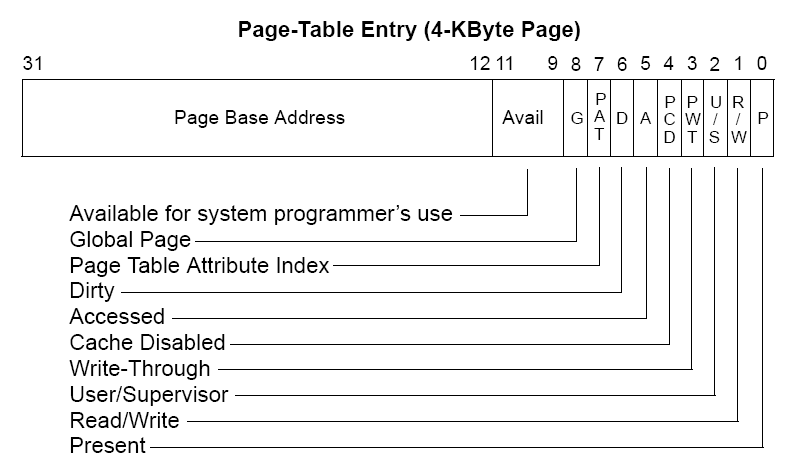
\includegraphics[width=0.47\textwidth]{figures/pte}
  \centering
  \caption{U/S, the 'User/Supervisor' bit, controls access to the page based on privilege level. If the bit is set, then this page is considered in user mode space and be accessed by all code; if the bit is not set, then it's considered in kernel mode space and can be accessed only by kernel mode code. }
  \label{fig:pte}
\end{figure}


When a page fault exception is raised, the faulting virtual address is always stored in the CR2(Control Register 2). To convert it to a kernel page, we simply locate it's PTE and set U/S bit to zero. It becomes part of the kernel space even though its address is not continuous with the traditional kernel address lower boundary such as 0x80000000. From this point, no other user-mode threads can access it, as shown in \autoref{fig:denyuserwrite}.

\begin{figure}[th]
  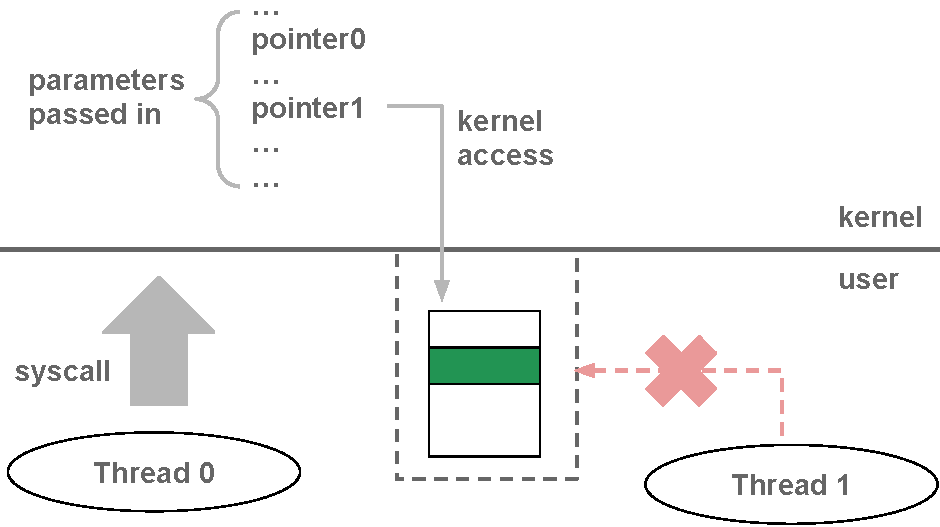
\includegraphics[width=0.47\textwidth]{figures/denyuserwrite}
  \centering
  \caption{}
  \label{fig:denyuserwrite}
\end{figure}

It's the basic model that sever the purpose of protecting user pages after kernel accesses them. Realistically, it's common that multiple threads access data that are located within the same page. For example, global data in the data segment, heap buffers and read-only data that merged with code, etc. One page being hold should not prevent other threads from reading it.


To address that issue, we extent the policy of page fault handling. When user-mode threads try to read a protected page, the fact that the page is now part of kernel space will trigger a page fault exception. Instead of terminating  the thread as the operating system would do, we take over the exception, change the page back to user-mode, plus making it as read-only, then let the thread re-executing the faulting instruction. The read access should be granted. \autoref{fig:pagestate} shows the page's attribute changes due to different accesses.
 

\begin{figure}[th]
  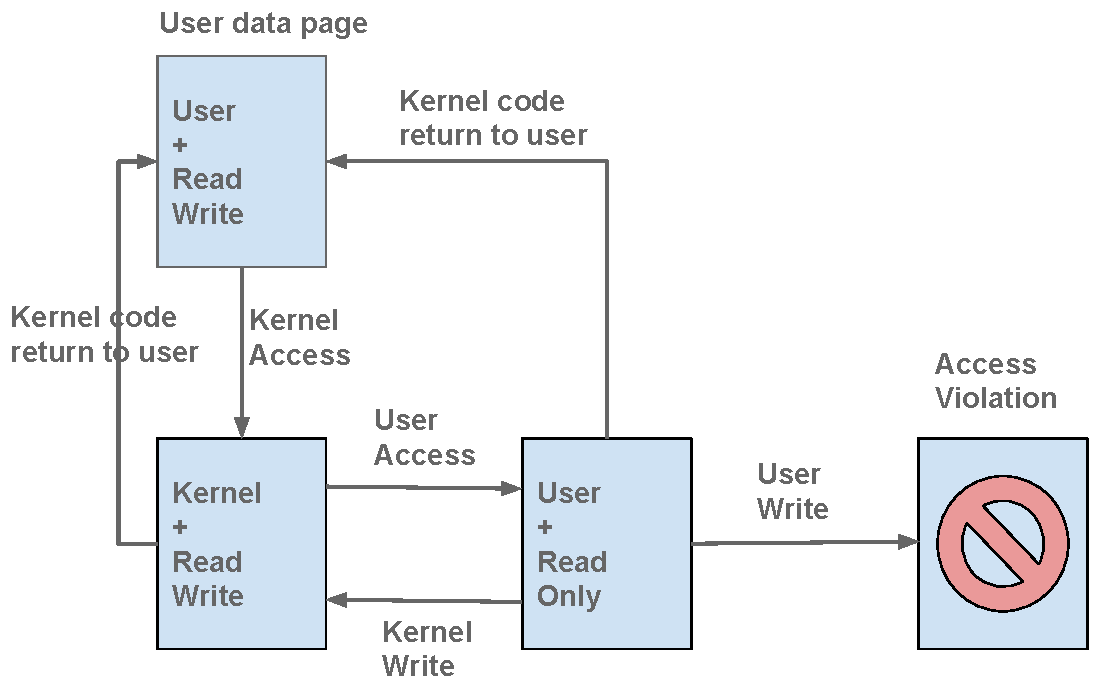
\includegraphics[width=0.45\textwidth]{figures/pagestate}
  \centering
  \caption{Page attributes transit between kernel mode and user mode. When kernel mode code ends, for example, system service returns to user mode, the page will be set back to the original permission}
  \label{fig:pagestate}
\end{figure}

As can be seen, the page either being part of the kernel space or stay read-only in user-mode. Meaning it can be read and written by kernel-mode code and be read by user-mode code. It only denies write accesses from user-mode, which is the root cause of kernel TOCTOU vulnerability.


There will also be write conflicts when pages are under protection. Due to the design of x86 architecture, it's difficult to isolate data for different threads in a more fine-gain granularity than page level. Allowing other user-mode threads to write the same page means losing security boundary. Since solving it does has practical significance, we propose a method that try to satisfy the writing thread from the time dimension.


\subsection{Solving Write Conflict }

For practical mitigations, compatibility is important. There are cases that program writes shared data or writes the data of the same page. Under the protection we just mentioned, such write access will trigger a page fault and causes thread exit. No synchronizing mechanism for shared resource, for example, user memory which is the root cause of kernel TOCTOU vulnerability. 

Since pages only be protected during the current system call, our solution is to hold the write thread, waiting for the system call to end. "Hold" means the write thread will give up it's time slice, letting operating system re-scheduling. 

\begin{figure}[th]
  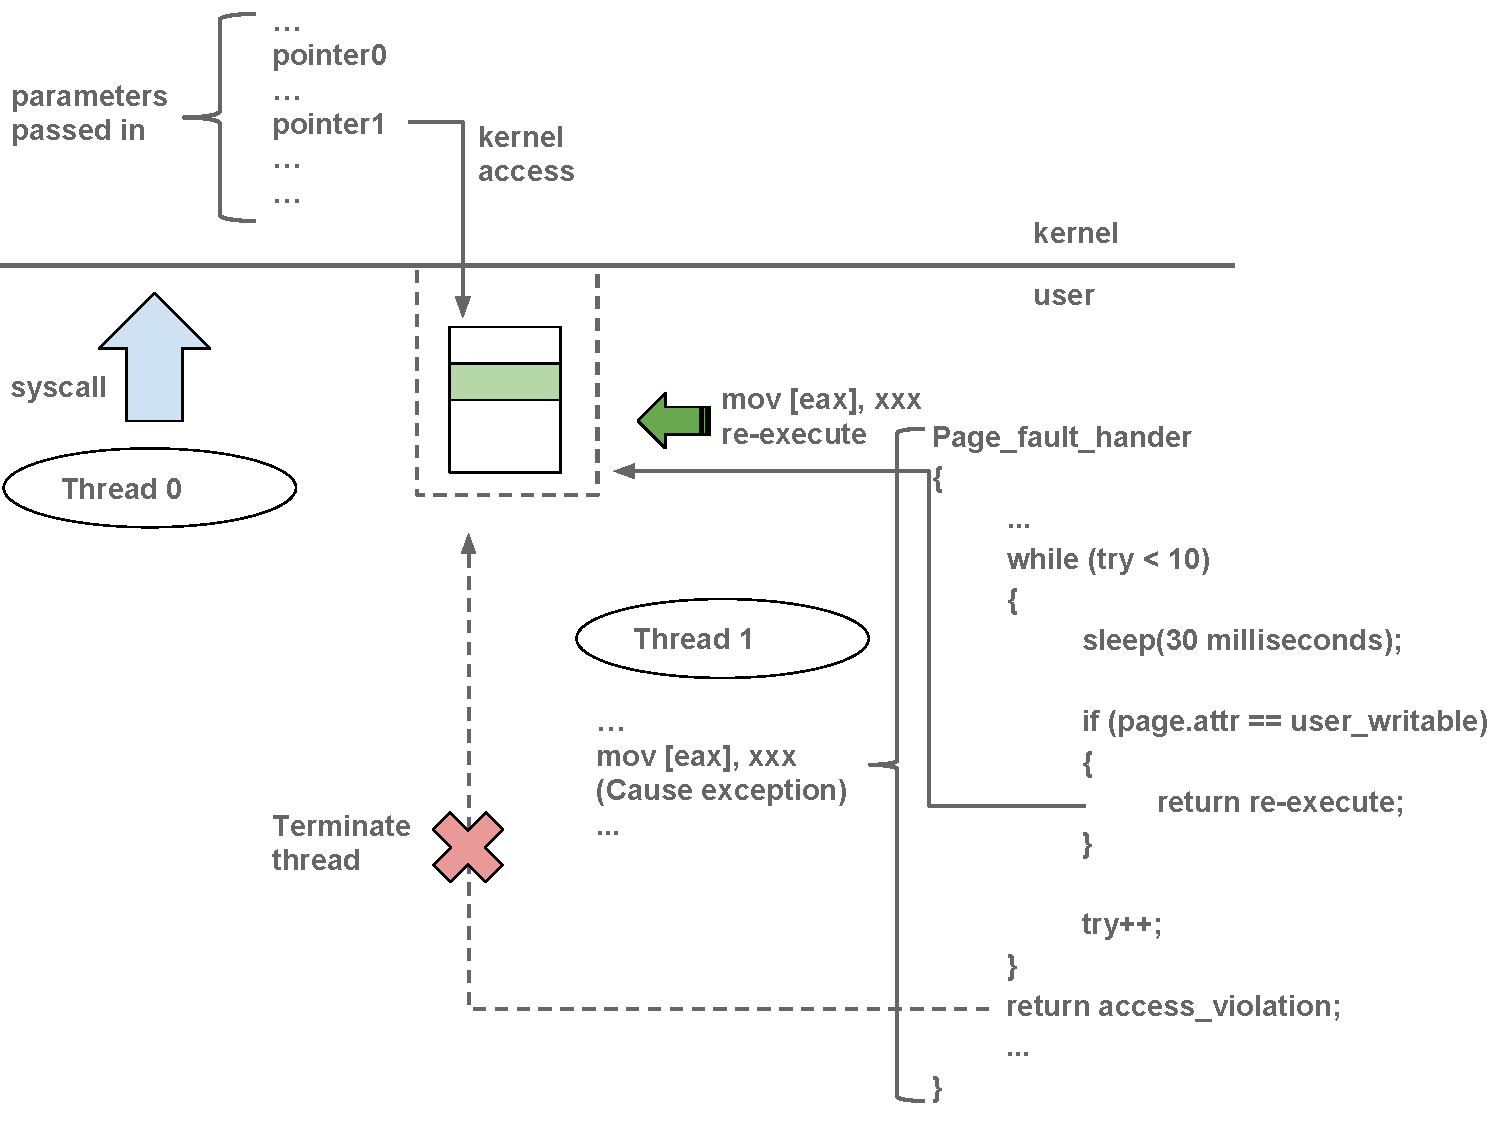
\includegraphics[width=0.47\textwidth]{figures/reexecute}
  \centering
  \caption{}
  \label{fig:reexecute}
\end{figure}

As shown in~\autoref{fig:reexecute}, Thread 1 is trying to access a protected page. Instead of terminating it, we hold it in the context of page fault exception, specifically, calling KeDelayExecutionThread() to put it to "sleep". But only for a certain amount of time, then it checks whether the page now is writable. If so, the page fault handler finish this exception and re-execute the fault instruction, otherwise, it waits for another round. A threshold is set to prevent infinite waiting. For example, after ten times, the thread will be terminated.

\subsubsection{Differences between Exception and Interruption}

To explain why thread can wait in the context of page fault exception, we briefly review the difference between exception and interruption of x86 architecture.

In x86 architecture, external(hardware) interrupts, software interrupts and exceptions are all handled through the interrupt descriptor table (IDT). 

External interrupt is a signal from a device such as network card, keyboards, telling CPU that an event just happened, need CPU to handle it immediately. External interrupts from different devices have different priorities, but mostly they have a higher priority than operating system thread scheduler. Meaning operating system need to handle external interrupt before any user-mode program, even most of the kernel code. To put the processor wait inside an external interrupt handler is not a good  practice, it extremely affects system performance. Operating system finishes external interrupts as soon as possible, even the lengthy low-priority part of a task is deferred for later execution. For example, in Windows operating system such mechanism is called DPC(Deferred Procedure Call). A single long-running deferred procedure call will be detected and raise a BugCheck (DPC\_WATCHDOG\_VIOLATION). DPCs should not run longer than 100 microseconds and ISRs should not run longer than 25 microseconds~\cite{msdnwatchdog}. In such environment, thread scheduling is not feasible.

Software Interrupt is an interrupt that signaled by software using "INT" instruction, such as "INT 0x2e", "INT 0x80" for system calls. 

What we leveraged in this project is exceptions. Exception is generated internally by the CPU to let the operating system handling an event or error such as double fault, page fault, general protection fault, etc. Different than external interruption, the priority of the exception handler is the same as the code that triggers the exception. Priority, in Windows operating system's term, is IRQL(Interrupt Request Level). When a user-mode program triggers a page fault exception, the control flow will be immediately transferred to the page fault handler which resides in the kernel, but the it's IRQL still stay at PASSIVE\_LEVEL which is the level where user program runs. Under PASSIVE\_LEVEL, thread scheduling is feasible.

\subsection{Releasing Protected Pages}

When a system call ends, all the related pages that being protected should be released. Their attributes will be restored which set free other waiting threads. There original attributes are recorded not only for restore purpose but also used as ground truth when to decide how to handle a page fault.


\begin{comment}
\begin{figure}[th]
  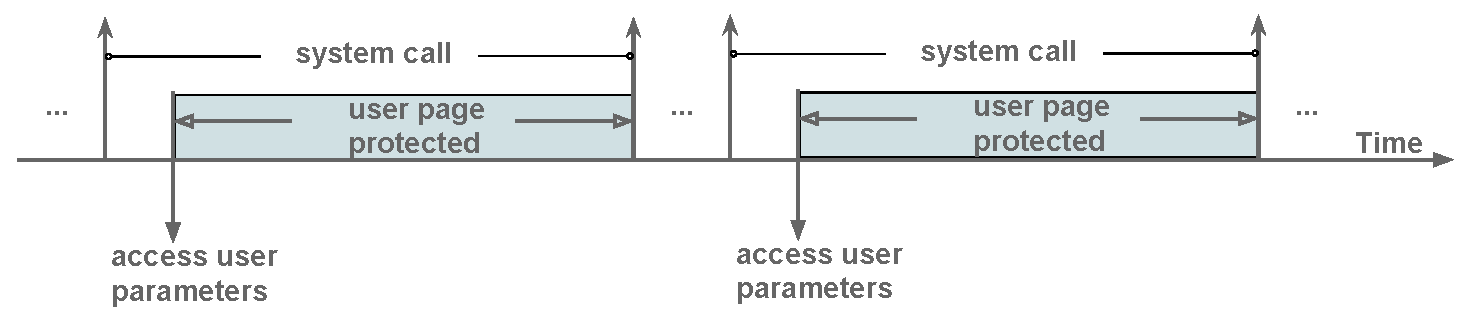
\includegraphics[width=0.47\textwidth]{figures/timeline}
  \centering
  \caption{The page protection period is within one system call cycle, this is based on the fact that kernel TOCTOU vulnerability does not happen across system calls.}
  \label{fig:timeline}
\end{figure}
\end{comment}


%We choose to install a hook near the end of system calls. On Windows operating system, such place could be, for example, KiServiceExit. Because during this function, Windows OS delivers pending APC~\cite{apc} which also needs to access user data. The hooking point that we choose is right after it calls KiDeliverAPC. It's not the very last instruction that the kernel mode execute, but we consider it close enough to the end of a system call.


Protected pages should be released according to specific thread. Meaning, when one thread finishes a system call, only those pages that related to itself should be released. To distinguish different thread in a process, TEB (Thread Environment Block~\cite{teb}) could be used as an identifier. TEB describes the state of a thread. Each thread has its own TEB structure and it's address can be found through segment register FS (at FS:0x18) which points to different locations for each thread. 

\subsection{Hypervisor}

SMAP is a system wide feature. Due to the way Windows kernel retrieve user-mode parameters (continuous read of one buffer may even cause a series of exceptions), huge amount of exception is expected. Also, SMAP caused exception needs proper handling, it can't be passed to operating system. Moreover, page fault is one of the core mechanism that builds up MMU of x86 architecture. Its handler is highly optimized to handle tremendous amount of exceptions, even a few more instructions introduced may affect system's performance.  To eliminate unnecessary system overhead, we provide a thin hypervisor that only enables SMAP on certain processes.

Not all the processes need to be monitored, such as the ones that already run with administrator or system privilege. Because kernel TOCTOU vulnerabilities are mostly used to escalate privilege. Normally, services that may potentially be controlled locally or remotely by attackers and alien processes are the suspects of privilege escalation attacks.

The hypervisor is simple and efficient. It's loaded as a Windows kernel driver at runtime, so the operating system doesn't need to change the way it boots. It only lifts the running operating system into VMM guest mode in order to intercept system events and change system's behavior. No hardware emulation is needed.  

\subsubsection{Process Context Switch}

One of the main character of virtual memory of x86 architecture is that each process has its own virtual address space which shared by multiple threads that exist within a process. Each process has a private set of page tables that represents the mappings between virtual memory and physical memory. Their root is stored in control register CR3. 

In Windows operating system, instead of process, thread is the base unit for task scheduling. But when scheduling to a thread of another process, the virtual address space needs to change too. Hence the changing of CR3 can be the indicator for process context switch. Fortunately, Intel's virtualizaton technology is able to capture the event.


\subsubsection{Virtualization Techniques}

"MOV from/to CR3" is one of the instructions that cause VM exits when they are executed in VMX non-root operation(guest mode). For example, "MOV CR3, EAX", where general register EAX contains the new page directory address, indicates an on going process context switch.

Our hypervisor handles VM exits and compare the new CR3 value with the ones that need to be monitored. If match, it sets the SMAP bit in the CR4 of VMCS(Virtual Machine Control Structure) so that when the VM resumes, the new value can be updated to the processor's CR4. Correspondingly, when the monitored processes are switched out, hypervisor does the opposite, clearing the SMAP bit. In such a way, the SMAP feature is only enabled in certain processes, as shown in~\autoref{fig:processsmap}.

\begin{figure}[th]
  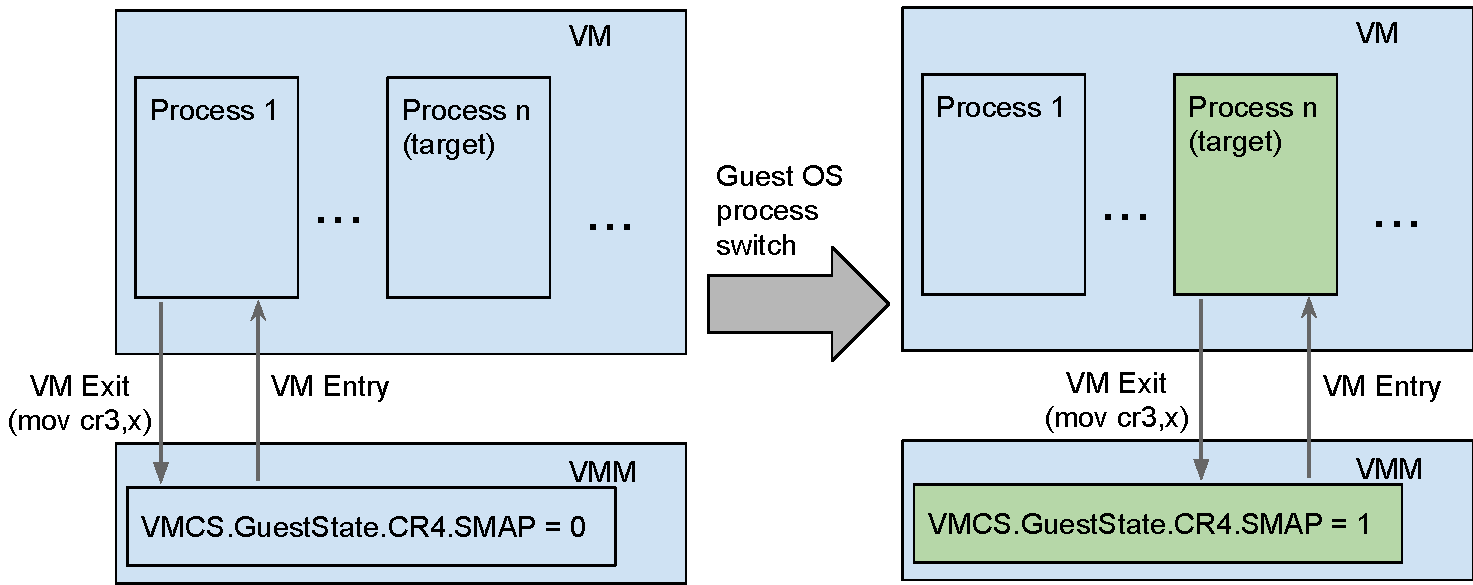
\includegraphics[width=0.47\textwidth]{figures/processsmap}
  \centering
  \caption{SMAP is only enabled on the target process. In other words, only target process can trigger SMAP exceptions.}
  \label{fig:processsmap}
\end{figure}
